\documentclass[twoside]{book}

% Packages required by doxygen
\usepackage{fixltx2e}
\usepackage{calc}
\usepackage{doxygen}
\usepackage[export]{adjustbox} % also loads graphicx
\usepackage{graphicx}
\usepackage[utf8]{inputenc}
\usepackage{makeidx}
\usepackage{multicol}
\usepackage{multirow}
\PassOptionsToPackage{warn}{textcomp}
\usepackage{textcomp}
\usepackage[nointegrals]{wasysym}
\usepackage[table]{xcolor}

% NLS support packages
Portuguese
% Font selection
\usepackage[T1]{fontenc}
\usepackage[scaled=.90]{helvet}
\usepackage{courier}
\usepackage{amssymb}
\usepackage{sectsty}
\renewcommand{\familydefault}{\sfdefault}
\allsectionsfont{%
  \fontseries{bc}\selectfont%
  \color{darkgray}%
}
\renewcommand{\DoxyLabelFont}{%
  \fontseries{bc}\selectfont%
  \color{darkgray}%
}
\newcommand{\+}{\discretionary{\mbox{\scriptsize$\hookleftarrow$}}{}{}}

% Page & text layout
\usepackage{geometry}
\geometry{%
  a4paper,%
  top=2.5cm,%
  bottom=2.5cm,%
  left=2.5cm,%
  right=2.5cm%
}
\tolerance=750
\hfuzz=15pt
\hbadness=750
\setlength{\emergencystretch}{15pt}
\setlength{\parindent}{0cm}
\setlength{\parskip}{3ex plus 2ex minus 2ex}
\makeatletter
\renewcommand{\paragraph}{%
  \@startsection{paragraph}{4}{0ex}{-1.0ex}{1.0ex}{%
    \normalfont\normalsize\bfseries\SS@parafont%
  }%
}
\renewcommand{\subparagraph}{%
  \@startsection{subparagraph}{5}{0ex}{-1.0ex}{1.0ex}{%
    \normalfont\normalsize\bfseries\SS@subparafont%
  }%
}
\makeatother

% Headers & footers
\usepackage{fancyhdr}
\pagestyle{fancyplain}
\fancyhead[LE]{\fancyplain{}{\bfseries\thepage}}
\fancyhead[CE]{\fancyplain{}{}}
\fancyhead[RE]{\fancyplain{}{\bfseries\leftmark}}
\fancyhead[LO]{\fancyplain{}{\bfseries\rightmark}}
\fancyhead[CO]{\fancyplain{}{}}
\fancyhead[RO]{\fancyplain{}{\bfseries\thepage}}
\fancyfoot[LE]{\fancyplain{}{}}
\fancyfoot[CE]{\fancyplain{}{}}
\fancyfoot[RE]{\fancyplain{}{\bfseries\scriptsize Gerado por Doxygen }}
\fancyfoot[LO]{\fancyplain{}{\bfseries\scriptsize Gerado por Doxygen }}
\fancyfoot[CO]{\fancyplain{}{}}
\fancyfoot[RO]{\fancyplain{}{}}
\renewcommand{\footrulewidth}{0.4pt}
\renewcommand{\chaptermark}[1]{%
  \markboth{#1}{}%
}
\renewcommand{\sectionmark}[1]{%
  \markright{\thesection\ #1}%
}

% Indices & bibliography
\usepackage{natbib}
\usepackage[titles]{tocloft}
\setcounter{tocdepth}{3}
\setcounter{secnumdepth}{5}
\makeindex

% Hyperlinks (required, but should be loaded last)
\usepackage{ifpdf}
\ifpdf
  \usepackage[pdftex,pagebackref=true]{hyperref}
\else
  \usepackage[ps2pdf,pagebackref=true]{hyperref}
\fi
\hypersetup{%
  colorlinks=true,%
  linkcolor=blue,%
  citecolor=blue,%
  unicode%
}

% Custom commands
\newcommand{\clearemptydoublepage}{%
  \newpage{\pagestyle{empty}\cleardoublepage}%
}

\usepackage{caption}
\captionsetup{labelsep=space,justification=centering,font={bf},singlelinecheck=off,skip=4pt,position=top}

%===== C O N T E N T S =====

\begin{document}

% Titlepage & ToC
\hypersetup{pageanchor=false,
             bookmarksnumbered=true,
             pdfencoding=unicode
            }
\pagenumbering{alph}
\begin{titlepage}
\vspace*{7cm}
\begin{center}%
{\Large Classes Abstratas \\[1ex]\large 1.\+0 }\\
\vspace*{1cm}
{\large Gerado por Doxygen 1.8.14}\\
\end{center}
\end{titlepage}
\clearemptydoublepage
\pagenumbering{roman}
\tableofcontents
\clearemptydoublepage
\pagenumbering{arabic}
\hypersetup{pageanchor=true}

%--- Begin generated contents ---
\chapter{Índice da hierarquia}
\section{Hierarquia de classes}
Esta lista de heranças está organizada, dentro do possível, por ordem alfabética\+:\begin{DoxyCompactList}
\item \contentsline{section}{Figura\+Geometrica}{\pageref{class_figura_geometrica}}{}
\begin{DoxyCompactList}
\item \contentsline{section}{Circulo}{\pageref{class_circulo}}{}
\item \contentsline{section}{Reta}{\pageref{class_reta}}{}
\item \contentsline{section}{Retangulo}{\pageref{class_retangulo}}{}
\end{DoxyCompactList}
\item \contentsline{section}{Screen}{\pageref{class_screen}}{}
\end{DoxyCompactList}

\chapter{Índice dos componentes}
\section{Lista de componentes}
Lista de classes, estruturas, uniões e interfaces com uma breve descrição\+:\begin{DoxyCompactList}
\item\contentsline{section}{\mbox{\hyperlink{class_circulo}{Circulo}} \\*A classe \mbox{\hyperlink{class_circulo}{Circulo}} é uma subclasse da \mbox{\hyperlink{class_figura_geometrica}{Figura\+Geometrica}} e serve para desenhar circunferência e círculos na tela }{\pageref{class_circulo}}{}
\item\contentsline{section}{\mbox{\hyperlink{class_figura_geometrica}{Figura\+Geometrica}} \\*A classe \mbox{\hyperlink{class_figura_geometrica}{Figura\+Geometrica}} serve para facilitar na construção das figuras geométricas }{\pageref{class_figura_geometrica}}{}
\item\contentsline{section}{\mbox{\hyperlink{class_reta}{Reta}} \\*A classe \mbox{\hyperlink{class_reta}{Reta}} é uma subclasse da \mbox{\hyperlink{class_figura_geometrica}{Figura\+Geometrica}} e desenha reta na tela }{\pageref{class_reta}}{}
\item\contentsline{section}{\mbox{\hyperlink{class_retangulo}{Retangulo}} \\*A classe \mbox{\hyperlink{class_retangulo}{Retangulo}} é uma subclasse da \mbox{\hyperlink{class_figura_geometrica}{Figura\+Geometrica}} e desenha retângulo na tela }{\pageref{class_retangulo}}{}
\item\contentsline{section}{\mbox{\hyperlink{class_screen}{Screen}} \\*A classe \mbox{\hyperlink{class_screen}{Screen}} é a tela a ser desenhada }{\pageref{class_screen}}{}
\end{DoxyCompactList}

\chapter{Documentação da classe}
\hypertarget{class_circulo}{}\section{Referência à classe Circulo}
\label{class_circulo}\index{Circulo@{Circulo}}


A classe \mbox{\hyperlink{class_circulo}{Circulo}} é uma subclasse da \mbox{\hyperlink{class_figura_geometrica}{Figura\+Geometrica}} e serve para desenhar circunferência e círculos na tela.  




{\ttfamily \#include $<$circulo.\+h$>$}

Diagrama de heranças da classe Circulo\begin{figure}[H]
\begin{center}
\leavevmode
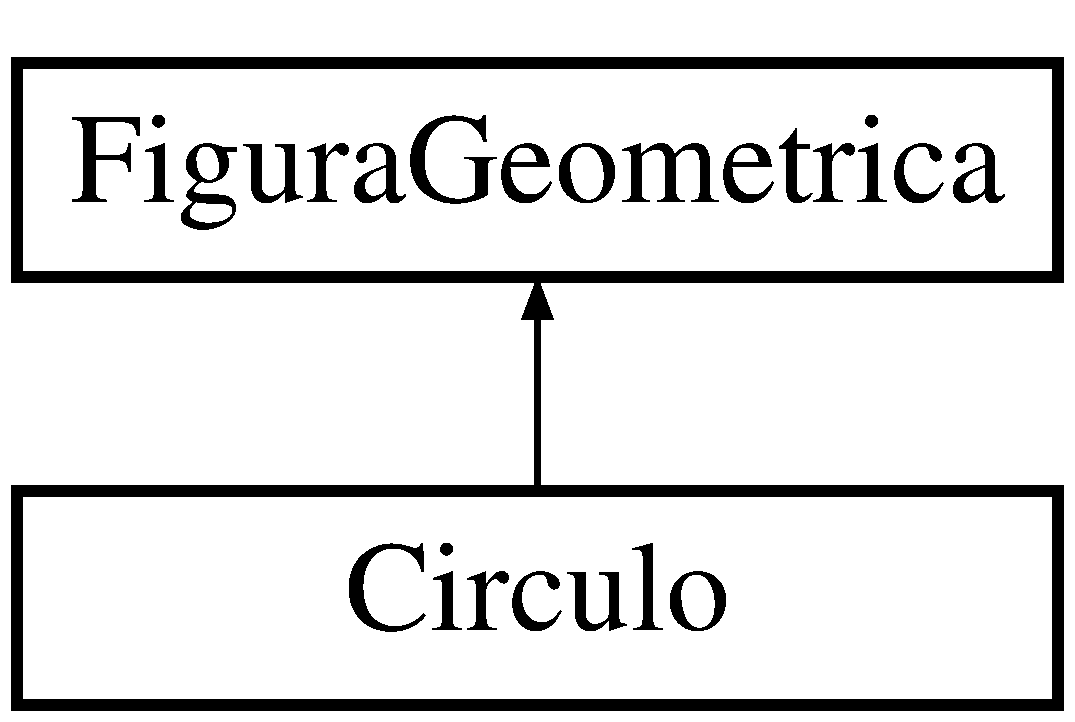
\includegraphics[height=2.000000cm]{class_circulo}
\end{center}
\end{figure}
\subsection*{Membros públicos}
\begin{DoxyCompactItemize}
\item 
\mbox{\hyperlink{class_circulo_a68c5a9226f3a366c5b92fc523e281fac}{Circulo}} (int \+\_\+xc, int \+\_\+yc, int \+\_\+raio, int fullmode, char \+\_\+brush)
\begin{DoxyCompactList}\small\item\em \mbox{\hyperlink{class_circulo}{Circulo}} \mbox{\hyperlink{class_circulo}{Circulo}} é o construtor da classe \mbox{\hyperlink{class_circulo}{Circulo}}. \end{DoxyCompactList}\item 
void \mbox{\hyperlink{class_circulo_a593787d6e0618c2eded23e8839e7bea6}{draw}} (\mbox{\hyperlink{class_screen}{Screen}} \&t)
\begin{DoxyCompactList}\small\item\em draw É uma função que permite desenhar na tela. \end{DoxyCompactList}\item 
void \mbox{\hyperlink{class_circulo_ae6d005ce309278d2f2ca170fdfa64e0a}{pontosdacircunferencia}} (int x, int y, \mbox{\hyperlink{class_screen}{Screen}} \&t)
\begin{DoxyCompactList}\small\item\em pontosdacircunferencia É a função que espelha os pontos do círculo \end{DoxyCompactList}\item 
void \mbox{\hyperlink{class_circulo_a4f0f6781f9ec3f501539f28a7788e9f1}{preencher}} (\mbox{\hyperlink{class_screen}{Screen}} \&t)
\begin{DoxyCompactList}\small\item\em preencher É a função que preenche a circuferência, transformando em círculo. \end{DoxyCompactList}\end{DoxyCompactItemize}


\subsection{Descrição detalhada}
A classe \mbox{\hyperlink{class_circulo}{Circulo}} é uma subclasse da \mbox{\hyperlink{class_figura_geometrica}{Figura\+Geometrica}} e serve para desenhar circunferência e círculos na tela. 

\subsection{Documentação dos Construtores \& Destrutor}
\mbox{\Hypertarget{class_circulo_a68c5a9226f3a366c5b92fc523e281fac}\label{class_circulo_a68c5a9226f3a366c5b92fc523e281fac}} 
\index{Circulo@{Circulo}!Circulo@{Circulo}}
\index{Circulo@{Circulo}!Circulo@{Circulo}}
\subsubsection{\texorpdfstring{Circulo()}{Circulo()}}
{\footnotesize\ttfamily Circulo\+::\+Circulo (\begin{DoxyParamCaption}\item[{int}]{\+\_\+xc,  }\item[{int}]{\+\_\+yc,  }\item[{int}]{\+\_\+raio,  }\item[{int}]{fullmode,  }\item[{char}]{\+\_\+brush }\end{DoxyParamCaption})}



\mbox{\hyperlink{class_circulo}{Circulo}} \mbox{\hyperlink{class_circulo}{Circulo}} é o construtor da classe \mbox{\hyperlink{class_circulo}{Circulo}}. 


\begin{DoxyParams}{Parâmetros}
{\em \+\_\+xc} & É a coordenada X do centro da circunferência ou círculo. \\
\hline
{\em \+\_\+yc} & É a coordenada Y do centro da circunferência ou círculo. \\
\hline
{\em \+\_\+raio} & É o tamanho do raio. \\
\hline
{\em fullmode} & Determinada se é círculo ou circunfêrencia. \\
\hline
{\em \+\_\+brush} & É o caractere a ser usado para desenhar. 
\begin{DoxyPre}
int main(void)\{
     \mbox{\hyperlink{class_circulo}{Circulo}} x(10,10,5,1,'+');
     return 0;
\}
\end{DoxyPre}
 \\
\hline
\end{DoxyParams}


\subsection{Documentação dos métodos}
\mbox{\Hypertarget{class_circulo_a593787d6e0618c2eded23e8839e7bea6}\label{class_circulo_a593787d6e0618c2eded23e8839e7bea6}} 
\index{Circulo@{Circulo}!draw@{draw}}
\index{draw@{draw}!Circulo@{Circulo}}
\subsubsection{\texorpdfstring{draw()}{draw()}}
{\footnotesize\ttfamily void Circulo\+::draw (\begin{DoxyParamCaption}\item[{\mbox{\hyperlink{class_screen}{Screen}} \&}]{t }\end{DoxyParamCaption})\hspace{0.3cm}{\ttfamily [virtual]}}



draw É uma função que permite desenhar na tela. 


\begin{DoxyParams}{Parâmetros}
{\em t} & É a tela. 
\begin{DoxyPre}
int main(void)\{
     \mbox{\hyperlink{class_circulo}{Circulo}} x(10,10,5,1,'+');
     \mbox{\hyperlink{class_screen}{Screen}} tela(20,20);
     x.draw(t);
     return 0;
\}
\end{DoxyPre}
 \\
\hline
\end{DoxyParams}


Implementa \mbox{\hyperlink{class_figura_geometrica_a8ee8dedc060b6059a805ea091aef2c41}{Figura\+Geometrica}}.

\mbox{\Hypertarget{class_circulo_ae6d005ce309278d2f2ca170fdfa64e0a}\label{class_circulo_ae6d005ce309278d2f2ca170fdfa64e0a}} 
\index{Circulo@{Circulo}!pontosdacircunferencia@{pontosdacircunferencia}}
\index{pontosdacircunferencia@{pontosdacircunferencia}!Circulo@{Circulo}}
\subsubsection{\texorpdfstring{pontosdacircunferencia()}{pontosdacircunferencia()}}
{\footnotesize\ttfamily void Circulo\+::pontosdacircunferencia (\begin{DoxyParamCaption}\item[{int}]{x,  }\item[{int}]{y,  }\item[{\mbox{\hyperlink{class_screen}{Screen}} \&}]{t }\end{DoxyParamCaption})}



pontosdacircunferencia É a função que espelha os pontos do círculo 


\begin{DoxyParams}{Parâmetros}
{\em x} & É a coordenada x do ponto. \\
\hline
{\em y} & É a coordenada y do ponto. \\
\hline
{\em t} & É tela. 
\begin{DoxyPre}
Essa função é auxiliar da função draw.
\end{DoxyPre}
 \\
\hline
\end{DoxyParams}
\mbox{\Hypertarget{class_circulo_a4f0f6781f9ec3f501539f28a7788e9f1}\label{class_circulo_a4f0f6781f9ec3f501539f28a7788e9f1}} 
\index{Circulo@{Circulo}!preencher@{preencher}}
\index{preencher@{preencher}!Circulo@{Circulo}}
\subsubsection{\texorpdfstring{preencher()}{preencher()}}
{\footnotesize\ttfamily void Circulo\+::preencher (\begin{DoxyParamCaption}\item[{\mbox{\hyperlink{class_screen}{Screen}} \&}]{t }\end{DoxyParamCaption})}



preencher É a função que preenche a circuferência, transformando em círculo. 


\begin{DoxyParams}{Parâmetros}
{\em t} & É a tela. 
\begin{DoxyPre}
Essa função é auxiliar da função draw.
\end{DoxyPre}
 \\
\hline
\end{DoxyParams}


A documentação para esta classe foi gerada a partir dos seguintes ficheiros\+:\begin{DoxyCompactItemize}
\item 
circulo.\+h\item 
circulo.\+cpp\end{DoxyCompactItemize}

\hypertarget{class_figura_geometrica}{}\section{Referência à classe Figura\+Geometrica}
\label{class_figura_geometrica}\index{Figura\+Geometrica@{Figura\+Geometrica}}


A classe \mbox{\hyperlink{class_figura_geometrica}{Figura\+Geometrica}} serve para facilitar na construção das figuras geométricas.  




{\ttfamily \#include $<$figurageometrica.\+h$>$}

Diagrama de heranças da classe Figura\+Geometrica\begin{figure}[H]
\begin{center}
\leavevmode
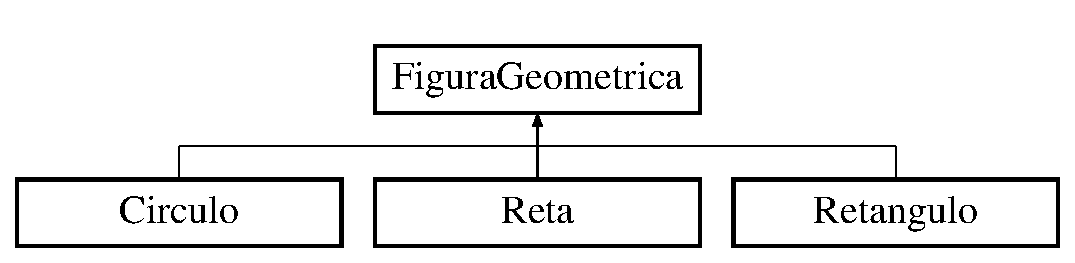
\includegraphics[height=2.000000cm]{class_figura_geometrica}
\end{center}
\end{figure}
\subsection*{Membros públicos}
\begin{DoxyCompactItemize}
\item 
virtual void \mbox{\hyperlink{class_figura_geometrica_a8ee8dedc060b6059a805ea091aef2c41}{draw}} (\mbox{\hyperlink{class_screen}{Screen}} \&t)=0
\begin{DoxyCompactList}\small\item\em draw É uma função virtual pura. \end{DoxyCompactList}\end{DoxyCompactItemize}


\subsection{Descrição detalhada}
A classe \mbox{\hyperlink{class_figura_geometrica}{Figura\+Geometrica}} serve para facilitar na construção das figuras geométricas. 

\subsection{Documentação dos métodos}
\mbox{\Hypertarget{class_figura_geometrica_a8ee8dedc060b6059a805ea091aef2c41}\label{class_figura_geometrica_a8ee8dedc060b6059a805ea091aef2c41}} 
\index{Figura\+Geometrica@{Figura\+Geometrica}!draw@{draw}}
\index{draw@{draw}!Figura\+Geometrica@{Figura\+Geometrica}}
\subsubsection{\texorpdfstring{draw()}{draw()}}
{\footnotesize\ttfamily virtual void Figura\+Geometrica\+::draw (\begin{DoxyParamCaption}\item[{\mbox{\hyperlink{class_screen}{Screen}} \&}]{t }\end{DoxyParamCaption})\hspace{0.3cm}{\ttfamily [pure virtual]}}



draw É uma função virtual pura. 


\begin{DoxyParams}{Parâmetros}
{\em t} & É a tela. \\
\hline
\end{DoxyParams}


Implementado em \mbox{\hyperlink{class_retangulo_ac088dd6d3f4f3d3f80363a868c2e74f1}{Retangulo}}, \mbox{\hyperlink{class_circulo_a593787d6e0618c2eded23e8839e7bea6}{Circulo}} e \mbox{\hyperlink{class_reta_ac2e9805183cd474b62bffd8b032cd780}{Reta}}.



A documentação para esta classe foi gerada a partir do seguinte ficheiro\+:\begin{DoxyCompactItemize}
\item 
figurageometrica.\+h\end{DoxyCompactItemize}

\hypertarget{class_reta}{}\section{Referência à classe Reta}
\label{class_reta}\index{Reta@{Reta}}


A classe \mbox{\hyperlink{class_reta}{Reta}} é uma subclasse da \mbox{\hyperlink{class_figura_geometrica}{Figura\+Geometrica}} e desenha reta na tela.  




{\ttfamily \#include $<$reta.\+h$>$}

Diagrama de heranças da classe Reta\begin{figure}[H]
\begin{center}
\leavevmode
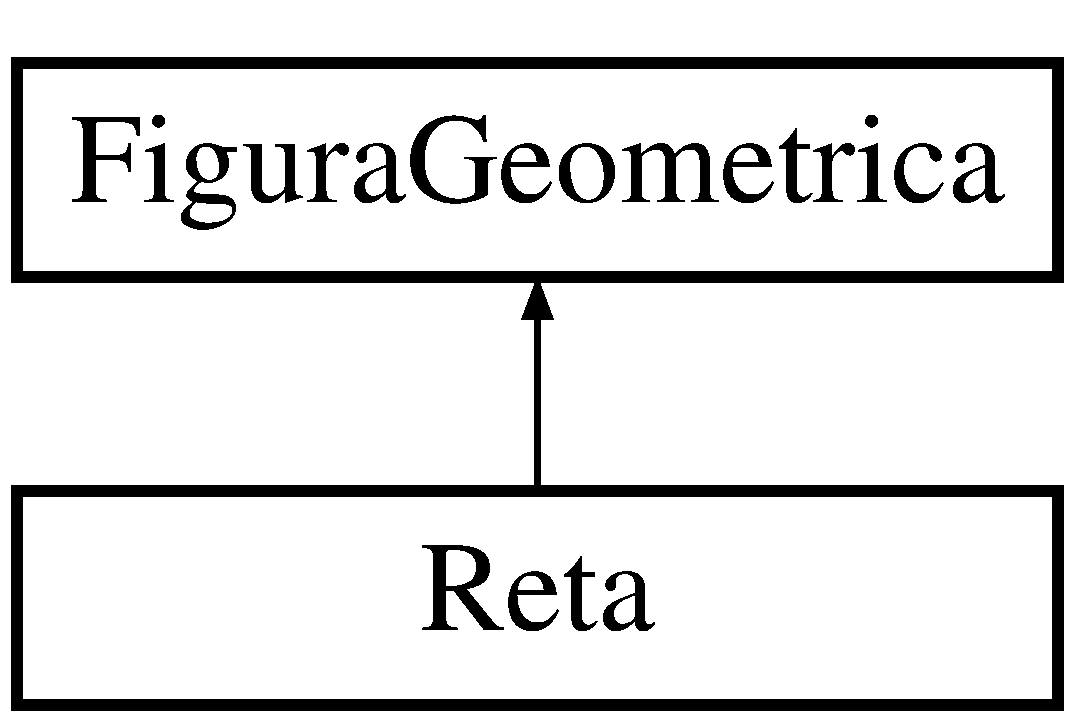
\includegraphics[height=2.000000cm]{class_reta}
\end{center}
\end{figure}
\subsection*{Membros públicos}
\begin{DoxyCompactItemize}
\item 
\mbox{\hyperlink{class_reta_aa399d9c0a34aafd01ce4017f49731148}{Reta}} (int \+\_\+xi, int \+\_\+yi, int \+\_\+xf, int \+\_\+yf, char \+\_\+brush)
\begin{DoxyCompactList}\small\item\em \mbox{\hyperlink{class_reta}{Reta}} É o construtor da classe \mbox{\hyperlink{class_reta}{Reta}}. \end{DoxyCompactList}\item 
void \mbox{\hyperlink{class_reta_ac2e9805183cd474b62bffd8b032cd780}{draw}} (\mbox{\hyperlink{class_screen}{Screen}} \&t)
\begin{DoxyCompactList}\small\item\em draw É uma função que permite desenhar na tela. \end{DoxyCompactList}\end{DoxyCompactItemize}


\subsection{Descrição detalhada}
A classe \mbox{\hyperlink{class_reta}{Reta}} é uma subclasse da \mbox{\hyperlink{class_figura_geometrica}{Figura\+Geometrica}} e desenha reta na tela. 

\subsection{Documentação dos Construtores \& Destrutor}
\mbox{\Hypertarget{class_reta_aa399d9c0a34aafd01ce4017f49731148}\label{class_reta_aa399d9c0a34aafd01ce4017f49731148}} 
\index{Reta@{Reta}!Reta@{Reta}}
\index{Reta@{Reta}!Reta@{Reta}}
\subsubsection{\texorpdfstring{Reta()}{Reta()}}
{\footnotesize\ttfamily Reta\+::\+Reta (\begin{DoxyParamCaption}\item[{int}]{\+\_\+xi,  }\item[{int}]{\+\_\+yi,  }\item[{int}]{\+\_\+xf,  }\item[{int}]{\+\_\+yf,  }\item[{char}]{\+\_\+brush }\end{DoxyParamCaption})}



\mbox{\hyperlink{class_reta}{Reta}} É o construtor da classe \mbox{\hyperlink{class_reta}{Reta}}. 


\begin{DoxyParams}{Parâmetros}
{\em \+\_\+xi} & É o x inicial da reta. \\
\hline
{\em \+\_\+yi} & É o y inicial da reta \\
\hline
{\em \+\_\+xf} & É o x final da reta. \\
\hline
{\em \+\_\+yf} & É o y final da reta. \\
\hline
{\em \+\_\+brush} & É o caractere a ser usado para desenhar. 
\begin{DoxyPre}
int main(void)\{
     \mbox{\hyperlink{class_reta}{Reta}} x(0,0,5,5,'*');
     return 0;
\}
\end{DoxyPre}
 \\
\hline
\end{DoxyParams}


\subsection{Documentação dos métodos}
\mbox{\Hypertarget{class_reta_ac2e9805183cd474b62bffd8b032cd780}\label{class_reta_ac2e9805183cd474b62bffd8b032cd780}} 
\index{Reta@{Reta}!draw@{draw}}
\index{draw@{draw}!Reta@{Reta}}
\subsubsection{\texorpdfstring{draw()}{draw()}}
{\footnotesize\ttfamily void Reta\+::draw (\begin{DoxyParamCaption}\item[{\mbox{\hyperlink{class_screen}{Screen}} \&}]{t }\end{DoxyParamCaption})\hspace{0.3cm}{\ttfamily [virtual]}}



draw É uma função que permite desenhar na tela. 


\begin{DoxyParams}{Parâmetros}
{\em t} & É a tela. 
\begin{DoxyPre}
int main(void)\{
     \mbox{\hyperlink{class_reta}{Reta}} x(0,0,5,5,'*');
     \mbox{\hyperlink{class_screen}{Screen}} tela(20,20);
     x.draw(tela);
     return 0;
\}
\end{DoxyPre}
 \\
\hline
\end{DoxyParams}


Implementa \mbox{\hyperlink{class_figura_geometrica_a8ee8dedc060b6059a805ea091aef2c41}{Figura\+Geometrica}}.



A documentação para esta classe foi gerada a partir dos seguintes ficheiros\+:\begin{DoxyCompactItemize}
\item 
reta.\+h\item 
reta.\+cpp\end{DoxyCompactItemize}

\hypertarget{class_retangulo}{}\section{Referência à classe Retangulo}
\label{class_retangulo}\index{Retangulo@{Retangulo}}


A classe \mbox{\hyperlink{class_retangulo}{Retangulo}} é uma subclasse da \mbox{\hyperlink{class_figura_geometrica}{Figura\+Geometrica}} e desenha retângulo na tela.  




{\ttfamily \#include $<$retangulo.\+h$>$}

Diagrama de heranças da classe Retangulo\begin{figure}[H]
\begin{center}
\leavevmode
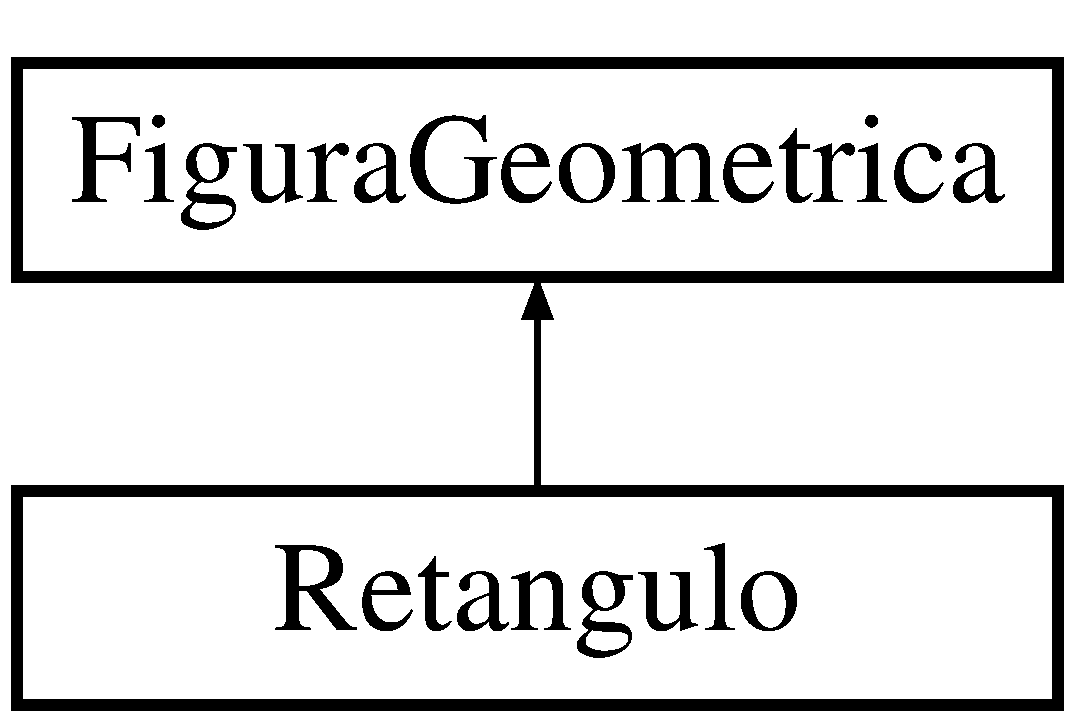
\includegraphics[height=2.000000cm]{class_retangulo}
\end{center}
\end{figure}
\subsection*{Membros públicos}
\begin{DoxyCompactItemize}
\item 
\mbox{\hyperlink{class_retangulo_a98680c1886ca4caccfe37f7084bbf499}{Retangulo}} (int \+\_\+xe, int \+\_\+ye, int \+\_\+larg, int \+\_\+alt, int fullmode, char \+\_\+brush)
\begin{DoxyCompactList}\small\item\em \mbox{\hyperlink{class_retangulo}{Retangulo}} É o construtor da classe \mbox{\hyperlink{class_retangulo}{Retangulo}}. \end{DoxyCompactList}\item 
void \mbox{\hyperlink{class_retangulo_ac088dd6d3f4f3d3f80363a868c2e74f1}{draw}} (\mbox{\hyperlink{class_screen}{Screen}} \&t)
\begin{DoxyCompactList}\small\item\em draw É a função para desenhar na tela. \end{DoxyCompactList}\end{DoxyCompactItemize}


\subsection{Descrição detalhada}
A classe \mbox{\hyperlink{class_retangulo}{Retangulo}} é uma subclasse da \mbox{\hyperlink{class_figura_geometrica}{Figura\+Geometrica}} e desenha retângulo na tela. 

\subsection{Documentação dos Construtores \& Destrutor}
\mbox{\Hypertarget{class_retangulo_a98680c1886ca4caccfe37f7084bbf499}\label{class_retangulo_a98680c1886ca4caccfe37f7084bbf499}} 
\index{Retangulo@{Retangulo}!Retangulo@{Retangulo}}
\index{Retangulo@{Retangulo}!Retangulo@{Retangulo}}
\subsubsection{\texorpdfstring{Retangulo()}{Retangulo()}}
{\footnotesize\ttfamily Retangulo\+::\+Retangulo (\begin{DoxyParamCaption}\item[{int}]{\+\_\+xe,  }\item[{int}]{\+\_\+ye,  }\item[{int}]{\+\_\+larg,  }\item[{int}]{\+\_\+alt,  }\item[{int}]{fullmode,  }\item[{char}]{\+\_\+brush }\end{DoxyParamCaption})}



\mbox{\hyperlink{class_retangulo}{Retangulo}} É o construtor da classe \mbox{\hyperlink{class_retangulo}{Retangulo}}. 


\begin{DoxyParams}{Parâmetros}
{\em \+\_\+xe} & É o x do canto superior esquerdo do retângulo. \\
\hline
{\em \+\_\+ye} & É o y do canto superior esquerdo da retângulo. \\
\hline
{\em \+\_\+larg} & É a largura do retângulo. \\
\hline
{\em \+\_\+alt} & É a altura do retângulo. \\
\hline
{\em fullmode} & Determinada se o retângulo será preenchido. \\
\hline
{\em \+\_\+brush} & É o caractere a ser usado para desenhar. 
\begin{DoxyPre}
int main (void)\{
     \mbox{\hyperlink{class_retangulo}{Retangulo}} x(0,0,5,5,1,'p');
     return 0;
\}
\end{DoxyPre}
 \\
\hline
\end{DoxyParams}


\subsection{Documentação dos métodos}
\mbox{\Hypertarget{class_retangulo_ac088dd6d3f4f3d3f80363a868c2e74f1}\label{class_retangulo_ac088dd6d3f4f3d3f80363a868c2e74f1}} 
\index{Retangulo@{Retangulo}!draw@{draw}}
\index{draw@{draw}!Retangulo@{Retangulo}}
\subsubsection{\texorpdfstring{draw()}{draw()}}
{\footnotesize\ttfamily void Retangulo\+::draw (\begin{DoxyParamCaption}\item[{\mbox{\hyperlink{class_screen}{Screen}} \&}]{t }\end{DoxyParamCaption})\hspace{0.3cm}{\ttfamily [virtual]}}



draw É a função para desenhar na tela. 


\begin{DoxyParams}{Parâmetros}
{\em t} & É a tela. 
\begin{DoxyPre}
int main (void)\{
     \mbox{\hyperlink{class_retangulo}{Retangulo}} x(0,0,5,5,1,'p');
     \mbox{\hyperlink{class_screen}{Screen}} tela(20,20);
     x.draw(tela);
     return 0;
\}
\end{DoxyPre}
 \\
\hline
\end{DoxyParams}


Implementa \mbox{\hyperlink{class_figura_geometrica_a8ee8dedc060b6059a805ea091aef2c41}{Figura\+Geometrica}}.



A documentação para esta classe foi gerada a partir dos seguintes ficheiros\+:\begin{DoxyCompactItemize}
\item 
retangulo.\+h\item 
retangulo.\+cpp\end{DoxyCompactItemize}

\hypertarget{class_screen}{}\section{Referência à classe Screen}
\label{class_screen}\index{Screen@{Screen}}


A classe \mbox{\hyperlink{class_screen}{Screen}} é a tela a ser desenhada.  




{\ttfamily \#include $<$screen.\+h$>$}

\subsection*{Membros públicos}
\begin{DoxyCompactItemize}
\item 
\mbox{\hyperlink{class_screen_a6c21beca43d25854d8674445127ef2eb}{Screen}} (int \+\_\+nlin, int \+\_\+ncol)
\begin{DoxyCompactList}\small\item\em \mbox{\hyperlink{class_screen}{Screen}} É o construtor da classe \mbox{\hyperlink{class_screen}{Screen}}. \end{DoxyCompactList}\item 
void \mbox{\hyperlink{class_screen_ae6bea81c57a22d226507c3c26fa95ee0}{set\+Pixel}} (int x, int y)
\begin{DoxyCompactList}\small\item\em set\+Pixel É uma função para desenhar na tela. \end{DoxyCompactList}\item 
void \mbox{\hyperlink{class_screen_a35e74266b2a04e37b354ceff7a5f1031}{clear}} ()
\begin{DoxyCompactList}\small\item\em clear É a função de limpar a tela. \end{DoxyCompactList}\item 
void \mbox{\hyperlink{class_screen_aebc4eb6cb5acf15a0f04c1494622ab23}{set\+Brush}} (char \+\_\+brush)
\begin{DoxyCompactList}\small\item\em set\+Brush É a função de mudar o caractere para desenho. \end{DoxyCompactList}\end{DoxyCompactItemize}
\subsection*{Amigos}
\begin{DoxyCompactItemize}
\item 
ostream \& \mbox{\hyperlink{class_screen_aab6a2880746bfe1b7964817cc8f0989e}{operator$<$$<$}} (ostream \&os, \mbox{\hyperlink{class_screen}{Screen}} \&t)
\begin{DoxyCompactList}\small\item\em operator $<$$<$ É o operador sobrecarregado para imprimir a tela no terminal. \end{DoxyCompactList}\end{DoxyCompactItemize}


\subsection{Descrição detalhada}
A classe \mbox{\hyperlink{class_screen}{Screen}} é a tela a ser desenhada. 

\subsection{Documentação dos Construtores \& Destrutor}
\mbox{\Hypertarget{class_screen_a6c21beca43d25854d8674445127ef2eb}\label{class_screen_a6c21beca43d25854d8674445127ef2eb}} 
\index{Screen@{Screen}!Screen@{Screen}}
\index{Screen@{Screen}!Screen@{Screen}}
\subsubsection{\texorpdfstring{Screen()}{Screen()}}
{\footnotesize\ttfamily Screen\+::\+Screen (\begin{DoxyParamCaption}\item[{int}]{\+\_\+nlin,  }\item[{int}]{\+\_\+ncol }\end{DoxyParamCaption})}



\mbox{\hyperlink{class_screen}{Screen}} É o construtor da classe \mbox{\hyperlink{class_screen}{Screen}}. 


\begin{DoxyParams}{Parâmetros}
{\em \+\_\+nlin} & É a quantidade de linhas da tela. \\
\hline
{\em \+\_\+ncol} & É a quantidade de colunas da tela. \\
\hline
\end{DoxyParams}


\subsection{Documentação dos métodos}
\mbox{\Hypertarget{class_screen_a35e74266b2a04e37b354ceff7a5f1031}\label{class_screen_a35e74266b2a04e37b354ceff7a5f1031}} 
\index{Screen@{Screen}!clear@{clear}}
\index{clear@{clear}!Screen@{Screen}}
\subsubsection{\texorpdfstring{clear()}{clear()}}
{\footnotesize\ttfamily void Screen\+::clear (\begin{DoxyParamCaption}{ }\end{DoxyParamCaption})}



clear É a função de limpar a tela. 


\begin{DoxyPre}
int main(void)\{
   \mbox{\hyperlink{class_screen}{Screen}} tela(20,20);
   tela.clear;
   return 0;
\}
\end{DoxyPre}
 \mbox{\Hypertarget{class_screen_aebc4eb6cb5acf15a0f04c1494622ab23}\label{class_screen_aebc4eb6cb5acf15a0f04c1494622ab23}} 
\index{Screen@{Screen}!set\+Brush@{set\+Brush}}
\index{set\+Brush@{set\+Brush}!Screen@{Screen}}
\subsubsection{\texorpdfstring{set\+Brush()}{setBrush()}}
{\footnotesize\ttfamily void Screen\+::set\+Brush (\begin{DoxyParamCaption}\item[{char}]{\+\_\+brush }\end{DoxyParamCaption})}



set\+Brush É a função de mudar o caractere para desenho. 


\begin{DoxyParams}{Parâmetros}
{\em \+\_\+brush} & É o novo caractere. 
\begin{DoxyPre}
int main(void)\{
   \mbox{\hyperlink{class_screen}{Screen}} tela(20,20);
   tela.setBrush('+');
   return 0;
\}
\end{DoxyPre}
 \\
\hline
\end{DoxyParams}
\mbox{\Hypertarget{class_screen_ae6bea81c57a22d226507c3c26fa95ee0}\label{class_screen_ae6bea81c57a22d226507c3c26fa95ee0}} 
\index{Screen@{Screen}!set\+Pixel@{set\+Pixel}}
\index{set\+Pixel@{set\+Pixel}!Screen@{Screen}}
\subsubsection{\texorpdfstring{set\+Pixel()}{setPixel()}}
{\footnotesize\ttfamily void Screen\+::set\+Pixel (\begin{DoxyParamCaption}\item[{int}]{x,  }\item[{int}]{y }\end{DoxyParamCaption})}



set\+Pixel É uma função para desenhar na tela. 


\begin{DoxyParams}{Parâmetros}
{\em x} & É a posição x a ser desenhada. \\
\hline
{\em y} & É a posição y a ser desenhada. 
\begin{DoxyPre}
int main(void)\{
   \mbox{\hyperlink{class_screen}{Screen}} tela(20,20);
   tela.setPixel(10,10);
   return 0;
\}
\end{DoxyPre}
 \\
\hline
\end{DoxyParams}


\subsection{Documentação das classes amigas e funções relacionadas}
\mbox{\Hypertarget{class_screen_aab6a2880746bfe1b7964817cc8f0989e}\label{class_screen_aab6a2880746bfe1b7964817cc8f0989e}} 
\index{Screen@{Screen}!operator$<$$<$@{operator$<$$<$}}
\index{operator$<$$<$@{operator$<$$<$}!Screen@{Screen}}
\subsubsection{\texorpdfstring{operator$<$$<$}{operator<<}}
{\footnotesize\ttfamily ostream\& operator$<$$<$ (\begin{DoxyParamCaption}\item[{ostream \&}]{os,  }\item[{\mbox{\hyperlink{class_screen}{Screen}} \&}]{t }\end{DoxyParamCaption})\hspace{0.3cm}{\ttfamily [friend]}}



operator $<$$<$ É o operador sobrecarregado para imprimir a tela no terminal. 


\begin{DoxyParams}{Parâmetros}
{\em os} & É o ostream de saída. \\
\hline
{\em t} & É a tela. \\
\hline
\end{DoxyParams}
\begin{DoxyReturn}{Retorna}
Retorna o endereço do ostream. 
\begin{DoxyPre}
int main(void)\{
   \mbox{\hyperlink{class_screen}{Screen}} tela(20,20);
   cout<<tela;
   return 0;
\}
\end{DoxyPre}
 
\end{DoxyReturn}


A documentação para esta classe foi gerada a partir dos seguintes ficheiros\+:\begin{DoxyCompactItemize}
\item 
screen.\+h\item 
screen.\+cpp\end{DoxyCompactItemize}

%--- End generated contents ---

% Index
\backmatter
\newpage
\phantomsection
\clearemptydoublepage
\addcontentsline{toc}{chapter}{Índice}
\printindex

\end{document}
